\RequirePackage[hyphens]{url}
\documentclass[hidelinks,a4paper,border=1pt]{standalone}
%% maxwidth is the original width if it is less than linewidth
%% otherwise use linewidth (to make sure the graphics do not exceed the margin)
\usepackage{amsmath}
\usepackage{graphicx}
\usepackage{url}
%\usepackage[hyphens]{url}
\usepackage{hyperref}
\usepackage{breakurl}
\usepackage{setspace}
\usepackage{array}
\usepackage{amssymb}
\usepackage[mathscr]{euscript}
%\renewcommand{\rmdefault}{bch} % change default font
\usepackage{tikz}
\usetikzlibrary{calc}
\usetikzlibrary{shapes}
\usepackage{enumitem}
\setlength{\parindent}{0in}
\usepackage{bm}
\usepackage{multirow}
\usepackage{adjustbox}
\usepackage{scalerel}
\usepackage[many]{tcolorbox}
\usepackage{booktabs}
\usepackage{float}
%\usepackage{adjustbox}
%>{\centering\arraybackslash}m{3cm}
%\newcolumntype{Y}{>{\small\raggedright\arraybackslash}X}
%\newcolumntype{C}{>{\centering\arraybackslash}m{3cm}}
\newcolumntype{C}{>{$}c<{$}}
%\captionsetup{
%	justification = centering
%}

\newcommand{\myfrac}[2]{\displaystyle \frac{#1}{#2}}
\newcommand{\dsum}{\displaystyle \sum}
%\newcommand{\mystrut}{\rule[10pt]{10pt}{20pt}}
\newcommand{\mystrut}{\rule[1\dp\strutbox]{0pt}{\baselineskip}}
\newcommand{\mysup}[1]{\scaleto{\rule[2.9\dp\strutbox]{0pt}{-1\baselineskip}^{#1}}{12pt}}
\newcommand{\mysub}[1]{\scaleto{\rule[-1.5\dp\strutbox]{-2.5pt}{-1\baselineskip}_{#1}}{5pt}}

% create "+" rule type for thick vertical lines
\newcolumntype{+}{!{\vrule width 2pt}}

% create \thickcline for thick horizontal lines of variable length
\newlength\savedwidth
\newcommand\thickcline[1]{%
	\noalign{\global\savedwidth\arrayrulewidth\global\arrayrulewidth 2pt}%
	\cline{#1}%
	\noalign{\vskip\arrayrulewidth}%
	\noalign{\global\arrayrulewidth\savedwidth}%
}

% \thickhline command for thick horizontal lines that span the table
\newcommand\thickhline{\noalign{\global\savedwidth\arrayrulewidth\global\arrayrulewidth 2pt}%
	\hline
	\noalign{\global\arrayrulewidth\savedwidth}}


% Remove comment for double spacing
%\usepackage{setspace} 
%\doublespacing

%\doublespacing
\pagenumbering{gobble}
\begin{document}

%\begin{table}[h!]
%\setlength\arrayrulewidth{1.2pt}
%\def\arraystretch{2}
%\centering
%\begin{tabular}{|>{\centering\arraybackslash}m{1.55cm}|>{\centering\arraybackslash}m{1cm}|>{\centering\arraybackslash}m{1.15cm}|>{\centering\arraybackslash}m{8.75cm}|@{}m{0pt}@{}}\hline 
%	{\bm{$q$}-\textbf{Metric}} & {\textbf{Data}} & {\textbf{Stat}} & {\textbf{Formula}} (\textbf{Eq.} \bm{$\#$}) & \\ \hline
%	\multirow{4}{*}[-2.8em]{\parbox{1.4cm}{standard (\textbf{Eq. 2})}} & $\mathcal{N}(0,1)$ & mean & $\left(\frac{2^q \Gamma\left(\frac{q+1}{2}\right)p}{\sqrt{\pi}}\right)^{1/q}$ (\textbf{38}) & \\ [1.5ex] \cline{2-4}
%	 & \vspace{0.3cm} $\mathcal{N}(0,1)$ & \vspace{0.3cm} variance & $\frac{4^q p}{q^2 \left(\frac{2^q \Gamma\left(\frac{q+1}{2}\right)}{\sqrt{\pi}}p\right)^{2\left(1 - \frac{1}{q}\right)}}\left[\frac{\Gamma\left(\frac{2q+1}{2}\right)}{\sqrt{\pi}} - \frac{\Gamma^2\left(\frac{q+1}{2}\right)}{\pi}\right]$  (\textbf{38}) & \\ [5ex] \cline{2-4}
%	 & $\mathcal{U}(0,1)$ & mean & $\left(\frac{2p}{(q+2)(q+1)}\right)^{1/q}$ \hspace{0.2cm} (\textbf{48}) & \\ [1.5ex] \cline{2-4}
%	 & \vspace{0.3cm} $\mathcal{U}(0,1)$ & \vspace{0.3cm} variance & $\frac{p}{q^2\left(\frac{2p}{(q+2)(q+1)}\right)^{2\left(1 - \frac{1}{q}\right)}}\left[\frac{1}{(q+1)(2q+1)} - \left(\frac{2}{(q+2)(q+1)}\right)^2\right]$ (\textbf{48}) & \\ [4ex] \hline
%	\multirow{4}{*}[-2.8em]{\parbox{1.54cm}{\hphantom{-}max-min \\ normalized \\ \hphantom{.}(\textbf{Eq. 59})}} & \vspace{0.3cm} $\mathcal{N}(0,1)$ & \vspace{0.3cm} mean & \parbox{8.75cm}{\centering $\frac{\mu_{D^{(q)}_{ij}}}{2\mu^{(1)}_\text{max}(m)}$ (\textbf{93}) \\ {\fontsize{7.5}{1}\selectfont where $\mu_{D^{(q)}_{ij}}$ and $\mu^{(1)}_{\text{max}(m)}$ are given by Eqs. 38 and 87, respectively.}} & \\ [3ex] \cline{2-4}
%	& & & & \\ [5ex] \cline{2-4}
%	& & & & \\ \cline{2-4}
%	& & & & \\ \hline
%\end{tabular}
%\end{table}

\begin{tikzpicture}
		
	% trim=left botm right top
	\node at (0,0) {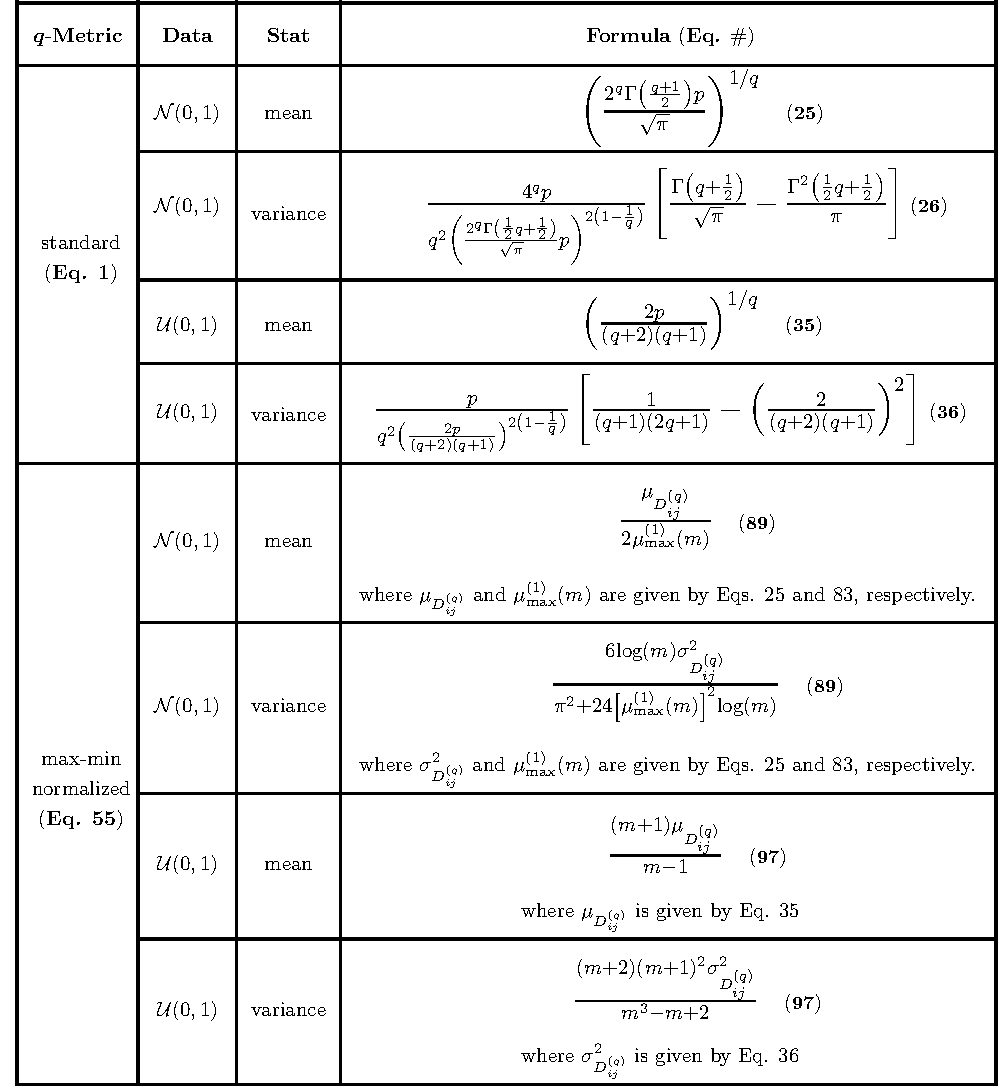
\includegraphics[clip,trim=0.27cm 0.0cm 0.0cm 0.05cm,width=\textwidth]{updated_distributions_table(5-23-2019).pdf}};

\end{tikzpicture}



\end{document}